\section{文本聚类技术的实现}

\subsection{聚类的概念}
聚类分析,是对一个未分组的样本集合进行分组的操作,它会将数据分组,组内相似度越大、组间的差别越大,那么聚类的效果越好。它应用于许多领域,包括机器学习、模式识别、图像分析、信息检索、生物信息学、数据压缩和计算机图形学。它是探索性数据挖掘的主要任务,也是统计数据分析的常用技术。

聚类不是一个特定的算法,而是解决此类问题的通用方案。它可以通过各种算法来实现,这些算法在实现类簇的构造以及如何有效地找到它们存在显着差异。主流的聚类概念包括簇内成员间距离最小的组,数据空间的密集区域,区间或特定的统计分布。因此,聚类可以转换为多目标最佳化问题。合适的聚类算法和参数设置(包括诸如要使用的距离函数,密度阈值或预期聚类的数量等参数)取决于单个数据集和结果的预期用途。这样的聚类分析不是自动执行的任务,而是在实验与失败的知识发现的过程中不断进行多目标优化的迭代过程。我们通常需要重跑数据预处理和调整模型参数,直到产出结果达到预期。

\begin{figure}[H]
	\begin{center}
		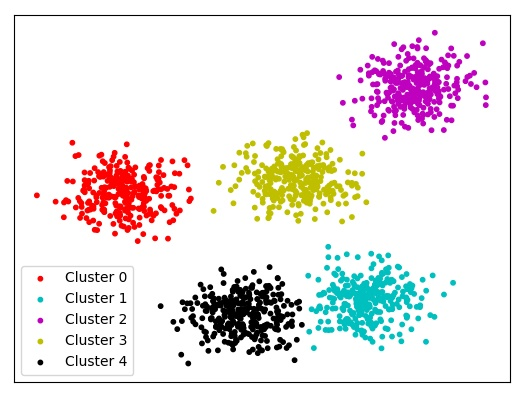
\includegraphics[width=1\linewidth]{cluster_result_graph.png}
	\end{center}
	\caption{聚类效果可视化}
	\label{word_vec:example}
\end{figure}

本论文使用的聚类算法为Kmeans算法和GSDMM算法

\subsection{使用的技术方法与工具}

\begin{table}[h!]
  \begin{center}
    \renewcommand\arraystretch{2}
    \begin{tabular}{|c|c|}
      \hline
      \textbf{参数} & \textbf{说明} \\
			\hline
			操作系统 & Ubuntu14.04.1 x86\_64 GNU/Linux  \\
			\hline
			编程语言 & Python 2.7.6 \\
			\hline
			虚拟环境管理器 & Pipenv version 2018.11.26 \\
			\hline
			\multirow{1}*{所使用包} & jieba-0.39\\
			~ & sklearn-0.20.3 \\
			~ & haha \\
			~ & haha \\

			\hline
    \end{tabular}
    \caption{Word2vec参数取值}
    \label{w2v_arg_table}
  \end{center}
\end{table} 